% coherence_mrf_deepdive.tex
% Deep dive on the Markov Random Field (MRF) formulation for logical coherence.
% Companion to coherence_modeling.tex and research_plan.md; focuses ONLY on the MRF.
% Compile: pdflatex coherence_mrf_deepdive.tex (run twice).
%
% All numeric marginals / Z / LCS values are EXACT (brute force over 2^16 worlds)
% for the AeroParts model, using FactReasoner's with-priors factor tables.

\documentclass[11pt]{article}

\usepackage[margin=1in]{geometry}
\usepackage{amsmath}
\usepackage{amssymb}
\usepackage{enumitem}
\usepackage{xcolor}
\usepackage{booktabs}
\usepackage{array}
\usepackage[numbers,square]{natbib}
\usepackage{tikz}
\usetikzlibrary{arrows.meta,positioning,calc,backgrounds,fit,shapes.geometric}
\usepackage[colorlinks=true,urlcolor=blue!60!black,linkcolor=blue!60!black,
            citecolor=blue!60!black]{hyperref}

\definecolor{cChain} {RGB}{210,228,248}
\definecolor{cEvid}  {RGB}{215,236,219}
\definecolor{cEquiv} {RGB}{226,221,243}
\definecolor{cConflA}{RGB}{248,205,205}
\definecolor{cConflB}{RGB}{249,222,229}
\definecolor{cHold}  {RGB}{250,219,180}
\definecolor{cFactor}{RGB}{60,60,60}

\tikzset{
  >={Stealth[length=2.4mm]},
  var/.style={draw,circle,minimum size=8.5mm,inner sep=0pt,
              font=\scriptsize\bfseries,fill=blue!6},
  varE/.style={var,fill=cEvid},
  varQ/.style={var,fill=cEquiv},
  varCA/.style={var,fill=cConflA},
  varCB/.style={var,fill=cConflB},
  varH/.style={var,fill=cHold,draw=orange!70!black,very thick},
  coh/.style={draw,rounded corners,minimum size=8.5mm,inner sep=1pt,
              font=\small\bfseries,fill=orange!25,draw=orange!70!black,very thick}, % reified R node
  fac/.style={draw,fill=black,minimum size=2.2mm,inner sep=0pt}, % factor square
  ufac/.style={fac,fill=gray!55},                                % unary factor
  efac/.style={fac,fill=blue!60!black},                          % entail factor
  qfac/.style={fac,fill=violet!60!black},                        % equiv factor
  cfac/.style={fac,fill=red!70!black},                           % contradiction factor
  xfac/.style={draw,fill=red!70!black,diamond,minimum size=2.9mm,inner sep=0pt}, % exclusive factor
  link/.style={-,gray!65,thick},
}

\title{The Markov Random Field Formulation of Logical Coherence\\
       \large Building the network from inter-atom relations, encoding discourse
       relations, and the Logical Coherence Score}
\author{FactReasoner --- Ideation}
\date{\today}

\begin{document}
\maketitle

\begin{abstract}\noindent
We commit to the undirected \textbf{Markov Random Field (MRF)} formulation and develop it
end to end: (i) how the Markov network is constructed from the mined inter-atom relations,
reusing FactReasoner's \texttt{MarkovNetwork} and factor tables; (ii) a two-level relation
scheme --- \emph{Level~1} inferential couplings that map directly to factors, and
\emph{Level~2} discourse relations that \emph{compile down} to Level~1 plus optional
structure; (iii) the \emph{AeroParts} running example, drawn as a factor graph;
(iv) a formal definition of the \textbf{Logical Coherence Score (LCS)}, choosing the
variant best suited to the MRF (the mean posterior marginal support); (v) a baseline
algorithm to compute it; and (vi) a coherent rewrite of the example showing exactly how the
LCS moves. All numbers are exact (brute force over $2^{16}$ worlds).
\end{abstract}

\tableofcontents

% =====================================================================================
\section{From relations to a Markov network}
\label{sec:build}

\subsection{Variables and the pairwise factorization}
The response is decomposed into atoms $A=\{a_1,\dots,a_n\}$, each a \emph{binary} random
variable ($a_i=1$: "the claim holds"; $a_i=0$: "it does not"). The relation miner returns a
set of directed, typed, weighted relations
\[
  R=\{\,r=(s,t,\tau,p)\,\},\qquad
  \tau\in\{\textsc{entail},\textsc{contradict},\textsc{equiv},\textsc{exclusive},\textsc{co-nec}\},\ \ p\in[0,1],
\]
where $s,t$ are the source/target atom ids, $\tau$ the Level-1 coupling
(Section~\ref{sec:level1}), and $p$ its confidence/strength (from
\texttt{-{}-nli-method\ logprobs} or \textbf{SIMBA-UQ} \citep{simbauq}). The MRF defines a
joint distribution as a normalized product of \emph{factors}:
\begin{equation}
  P(\mathbf a)\;=\;\frac{1}{Z}\;
  \underbrace{\prod_{i=1}^{n}\phi_i(a_i)}_{\text{unary priors}}\;
  \underbrace{\prod_{r\in R}\psi_r(a_{s_r},a_{t_r})}_{\text{pairwise relation factors}},
  \qquad
  Z=\sum_{\mathbf a}\prod_i\phi_i\prod_r\psi_r .
  \label{eq:joint}
\end{equation}
This is exactly the object built by
\texttt{assessor.py::\_build\_markov\_network}: one unary factor per node and one pairwise
factor per edge, serialized to UAI and solved by Merlin. The only change from the factuality
pipeline is that edges now connect \emph{atoms to atoms}
(\texttt{Edge.link="atom\_atom"}, already permitted by \texttt{fact\_graph.py}).

\subsection{Unary prior factors}
Each atom gets a prior factor
\(
  \phi_i(a_i)=[\,1-\pi_i,\ \pi_i\,]
\)
over states $(a_i{=}0,\,a_i{=}1)$. For \emph{coherence-only} analysis we use an uninformative
$\pi_i=0.5$ (we are asking whether the atoms \emph{hang together}, not whether they are
externally true). For a \emph{joint} factuality+coherence model, set $\pi_i$ to the atom's
factuality support score and keep the context nodes --- the same network then reflects both
axes.

\subsection{Pairwise relation factors (the exact tables)}
\label{sec:tables}
Each relation contributes a $2\times2$ factor $\psi_r$, laid out \emph{row-major over}
$[\text{src},\text{trg}]$, i.e.\ value order
$(0,0),(0,1),(1,0),(1,1)$. FactReasoner ships two variants
(\texttt{\_edge\_factor\_values}); the choice is the central modeling decision for
coherence.

\begin{table}[h]\centering\small
\renewcommand{\arraystretch}{1.25}
\begin{tabular}{@{}lcc@{}}
\toprule
$\tau$ & \textbf{no-priors} (atom$\leftrightarrow$context default)
       & \textbf{with-priors} (\textbf{use this} for atom$\leftrightarrow$atom)\\
\midrule
\textsc{entail}     & $[\,p,\ p,\ 1{-}p,\ p\,]$ & $[\,1{-}\pi_s,\ \pi_s,\ 1{-}p,\ p\,]$\\
\textsc{contradict} & $[\,p,\ p,\ p,\ 1{-}p\,]$ & $[\,1{-}\pi_s,\ \pi_s,\ p,\ 1{-}p\,]$\\
\textsc{equiv}      & $[\,p,\ 1{-}p,\ 1{-}p,\ p\,]$ & $[\,p,\ 1{-}p,\ 1{-}p,\ p\,]$\\
\textsc{exclusive}  & $[\,1{-}p,\ p,\ p,\ 1{-}p\,]$ & $[\,1{-}p,\ p,\ p,\ 1{-}p\,]$\\
\textsc{co-nec}     & $[\,1{-}p,\ p,\ p,\ p\,]$ & $[\,1{-}p,\ \pi_s,\ \pi_s,\ p\,]$\\
\bottomrule
\end{tabular}
\caption{Pairwise factor tables for the five Level-1 couplings. Reading, e.g., \textsc{entail}
with-priors: if the source is false the factor is the source prior $[\,1{-}\pi_s,\pi_s\,]$
(the implication says nothing); if the source is true, the target is pushed to $p$ (cell
$(1,1){=}p$) and away from $1{-}p$ (cell $(1,0)$). \textsc{exclusive} (exactly-one) penalizes
\emph{both} same-value worlds $(0,0)$ and $(1,1)$; \textsc{co-nec} (at-least-one) penalizes
only $(0,0)$. The last two are new (Section~\ref{sec:level1}); \textsc{exclusive} and
\textsc{equiv} share their symmetric form up to the sign of the interaction.}
\label{tab:tables}
\end{table}

\paragraph{Why with-priors for coherence.} The no-priors \textsc{entail} table charges the
\emph{source} being true whenever the target is uncertain (cell $(1,0){=}1{-}p$). That is
correct for atom$\leftrightarrow$\emph{context} factuality --- an atom with no supporting
context \emph{should} be pulled down --- but wrong for coherence, where a well-supported
\emph{premise} must not be penalized for being a premise. Exact inference confirms the
failure: under no-priors the backbone root $a_1$ collapses to $P(a_1){=}0.19$ and mean
support stays $0.46$ even after removing every contradiction. The with-priors tables
decouple the source's own probability from the implication and behave correctly
(Section~\ref{sec:example}). \textbf{We adopt the with-priors tables with $\pi_s=0.5$.}

% =====================================================================================
\section{Level 1: inferential couplings}
\label{sec:level1}

Level~1 is the set of couplings the MRF understands. The first three are FactReasoner's NLI
edge types; a coupling is fully characterized by which world(s) its $2\times2$ factor
penalizes, and enumerating the corners gives two more that cost only a new table (both
already inside the pairwise family --- see the coupling-vocabulary analysis in the companion
\texttt{coherence\_mln\_deepdive}). Each maps to one row of Table~\ref{tab:tables}.

\begin{itemize}[leftmargin=*]
  \item \textbf{\textsc{entail}} $s\!\Rightarrow\!t$ --- source true makes target true.
        Encodes prerequisite, cause$\to$effect, evidence, and subsumption. Directed:
        the factor is asymmetric ($(1,0)\neq(0,1)$); penalizes the world $(1,0)$.
  \item \textbf{\textsc{contradict}} $s\!\Rightarrow\!\neg t$ --- source true makes target
        false. Encodes contrast and position invalidation. The factor down-weights the
        $(1,1)$ cell to $1-p$: both-true is the incoherent configuration.
  \item \textbf{\textsc{equiv}} $s\!\Leftrightarrow\!t$ --- the two agree. Encodes
        restatement and mutual entailment. Symmetric: rewards $(0,0)$ and $(1,1)$, penalizes
        disagreement (the off-diagonal $s\neq t$).
  \item \textbf{\textsc{exclusive}} --- \emph{exactly one} of $s,t$ holds. Symmetric;
        penalizes \emph{both} same-value worlds $(0,0)$ and $(1,1)$. Encodes genuine
        alternatives (competing hypotheses, incompatible values of one slot) that are not
        only mutually exclusive but \emph{exhaustive}. It is \textsc{equiv} with the sign of
        the interaction flipped, and strictly stronger than \textsc{contradict} (which forbids
        only $(1,1)$).
  \item \textbf{\textsc{co-nec}} --- \emph{at least one} of $s,t$ holds. Symmetric; penalizes
        only the both-false world $(0,0)$. Encodes a disjunction or a joint prerequisite
        (``at least one of the two supporting findings must hold'').
  \item \textbf{\textsc{none}} --- no factor (atoms independent given the rest).
\end{itemize}

\paragraph{A standalone \textsc{co-nec} illustration.} \textsc{co-nec} has no natural home in
the AeroParts example (Section~\ref{sec:example}), so consider it in isolation. Two claims
$b_1$ ``the defect was detected by vibration analysis'' and $b_2$ ``the defect was detected by
metallurgical assay'' back a conclusion; the text asserts \emph{at least one} detection method
found it. With the with-priors table $[\,1{-}p,\ \pi_s,\ \pi_s,\ p\,]$ at $p{=}0.9$,
$\pi_s{=}0.5$, the both-false world $(0,0)$ carries mass $0.1$ against $0.5,0.5,0.9$ for the
others (normalized $0.05\,/\,0.25\,/\,0.25\,/\,0.45$): the joint denial of both methods is
suppressed while any single detection, or both, is fine. This is the positive-disjunction
mirror of \textsc{exclusive}.

At Level~1 the pipeline is complete: mine $\tau$ and $p$ for candidate atom pairs, drop
\textsc{none}, emit one factor each. These five couplings yield a working coherence model;
Level~2 adds interpretability and better strengths on top.

% =====================================================================================
\section{Level 2: encoding discourse relations}
\label{sec:level2}

Level~2 is the interpretable discourse inventory (PDTB~3.0 top classes \citep{pdtb3} and
RST \citep{rst}); a shallow discourse parser such as DiscoPrompt \citep{discoprompt} outputs
these. A Level-2 relation is not a new factor type --- it \emph{compiles} to Level~1 via a
deterministic rule
\(
  \mathcal C:\ \text{(discourse sense)}\ \mapsto\ (\tau,\ \text{strength prior},\ \text{aux structure}).
\)

\begin{table}[h]\centering\small
\renewcommand{\arraystretch}{1.15}
\begin{tabular}{@{}p{2.3cm}p{3.2cm}p{2.0cm}p{5.6cm}@{}}
\toprule
\textbf{PDTB top} & \textbf{Level-2 sense} & \textbf{$\to$ Level 1} & \textbf{Encoding in the MRF}\\
\midrule
Contingency & Cause-Effect / Effect-Cause & \textsc{entail} & one \textsc{entail} factor $s\!\to\!t$; $p$ $=$ causal plausibility (often $<1$)\\
Contingency & Evidence & \textsc{entail} & \textsc{entail} from evidence atom to claim\\
Contingency & Condition & \textsc{entail} & \textsc{entail} antecedent$\to$consequent\\
Comparison  & Contrast (non-exhaustive) & \textsc{contradict} & one \textsc{contradict} factor; $p$ $=$ conflict confidence\\
Comparison  & \textbf{Alternative} (exhaustive) & \textsc{exclusive} & one \textsc{exclusive} factor; the two are exclusive \emph{and} exhaustive (exactly one holds)\\
Comparison  & \textbf{Concession} & \textsc{contradict}/\textsc{exclusive} \emph{(discounted)} & the conflict factor whose $p$ is \emph{reduced} when a resolving atom is present (below)\\
Expansion   & Restatement & \textsc{equiv} & one \textsc{equiv} factor, high $p$\\
Expansion   & Instantiation / Subsumption & \textsc{entail} & \textsc{entail} general$\to$specific (or specific$\to$general)\\
Expansion   & \textbf{Disjunction} (at least one) & \textsc{co-nec} & one \textsc{co-nec} factor; at least one of the disjuncts holds\\
Temporal    & Precedence / Succession & \textsc{none} $+$ order & no truth coupling; record order for the invalidation direction\\
\bottomrule
\end{tabular}
\caption{Compiling Level-2 discourse senses to Level-1 factors (now five couplings). The map
carries a \emph{strength prior} (e.g.\ Restatement starts near $p{=}0.9$, a Cause-Effect at
the miner's confidence) that the confidence estimate then refines. A Comparison sense compiles
to \textsc{contradict} when the two claims are merely incompatible, and to \textsc{exclusive}
when they are \emph{exhaustive} alternatives (exactly one is true) --- the AeroParts casualty
and blame conflicts are of the latter kind (Section~\ref{sec:example}).}
\label{tab:compile}
\end{table}

\paragraph{The one structural case: Concession / resolved tension.}
A Concession (``although $X$, still $Y$'') or an adjudicating \emph{holding} is not a
coherence defect --- it is a conflict the text \emph{itself resolves}, and must be
discounted. In the MRF we encode this by letting the resolving atom modulate the conflict
factor's strength (whether that factor is a \textsc{contradict} or, as with the AeroParts
blame conflict, an \textsc{exclusive}). Concretely, for a conflict factor on $(s,t)$ that a
holding atom $h$ resolves, set
\begin{equation}
  p_{\text{eff}}(s,t)\;=\;p_{\text{raw}}(s,t)\cdot\big(1-\lambda\,\pi_h\big),
  \label{eq:concession}
\end{equation}
where $\pi_h$ is the holding's prior/belief and $\lambda\in[0,1]$ the discount. When the
holding is believed ($\pi_h\!\to\!1$) the contradiction softens toward neutral; when it is
absent the raw conflict stands. (Section~\ref{sec:example} uses a fixed
$p_{\text{raw}}{=}0.80 \to p_{\text{eff}}{=}0.55$.) This is the MRF's approximation of what a
Markov Logic Network would express as a cancel rule; keeping it as a strength discount lets
us stay entirely within the shipped pairwise machinery.

% =====================================================================================
\section{Estimating the relation probabilities with an LLM}
\label{sec:estimate}

Every factor in the network (Section~\ref{sec:tables}) is parameterized by a single number
$p\in[0,1]$ --- the confidence/strength of the relation. This section proposes a concrete
LLM-based method for producing those numbers, extending FactReasoner's existing NLI
extractor (\texttt{core/nli.py}) from the atom$\leftrightarrow$context factuality setting to
the two-level atom$\leftrightarrow$atom coherence setting of
Sections~\ref{sec:level1}--\ref{sec:level2}.

\subsection{What must be estimated}
For an ordered atom pair $(a_i,a_j)$ the miner must return three things:
\begin{enumerate}[leftmargin=*,nosep]
  \item the \textbf{Level-2 discourse sense} $\sigma\in\{$Cause-Effect, Evidence,
        Restatement, Contrast, Concession, \dots, \textsc{none}$\}$ (for interpretability
        and for the concession handling of Eq.~\ref{eq:concession});
  \item the \textbf{Level-1 coupling} $\tau\in\{\textsc{entail},\textsc{contradict},
        \textsc{equiv},\textsc{none}\}$ (which factor table to instantiate); and
  \item the \textbf{probability} $p$ that becomes the factor strength.
\end{enumerate}
Crucially, $p$ is the \emph{product of two distinct quantities}
(cf.\ the type-posterior$\times$conditional-strength decomposition):
\begin{equation}
  p \;=\; \underbrace{P(\tau \mid a_i,a_j)}_{\text{\emph{type} confidence:}}
          \;\times\;
          \underbrace{P(a_j \mid a_i,\tau)}_{\text{\emph{strength}:}}
  \qquad
  \begin{array}{l}\text{how sure the coupling is }\tau,\\[-1pt]
  \text{how strongly $a_i$ forces $a_j$ under }\tau.\end{array}
  \label{eq:pdecomp}
\end{equation}
The first factor guards against a confidently-stated but mis-typed relation; the second
captures that a \emph{plausible} cause-effect ($p{\approx}0.6$) should not enter the network
with the same strength as a near-certain restatement ($p{\approx}0.95$). Both are elicited
from the LLM.

\subsection{Prompt A --- joint sense + coupling classification (chain-of-thought)}
The primary call mirrors the shipped NLI prompt (\texttt{core/nli.py}: instruction $+$
few-shot $+$ bracketed final answer $+$ optional JSON), but (i) generalizes the three NLI
labels to the two-level scheme and (ii) asks for the discourse sense first, then the
coupling it compiles to. The chain-of-thought step matters: it is what makes the
\emph{type} confidence in Eq.~\eqref{eq:pdecomp} readable from the label logprobs, because
the model commits to the sense only after reasoning.

\begin{figure}[h]\centering
\fbox{\parbox{0.95\textwidth}{\footnotesize\ttfamily
\textbf{[system]}\ You are given two atomic claims A and B from the SAME response, in their
order of appearance. Decide the discourse/logical relation FROM A TO B.\\[4pt]
1. Reason step by step: does A cause, enable, provide evidence for, restate, elaborate,
temporally precede, contrast with, or contradict B? Is B a claim the text later withdraws or
that a holding resolves?\\
2. Name the DISCOURSE SENSE (one of: Cause-Effect, Effect-Cause, Evidence, Condition,
Restatement, Elaboration, Instantiation, Precedence, Succession, Contrast, Concession,
None).\\
3. Map it to a COUPLING: entailment / contradiction / equivalence / none.\\
4. Give your final answer as bracketed tags on one line, sense first:\\
\ \ \ \ [sense=Cause-Effect] [coupling=entailment]\\
A JSON object \{"sense":"Cause-Effect","coupling":"entailment"\} is also acceptable.\\[4pt]
\textbf{[few-shot examples]}\ (3--5, mirroring core/nli.py; each shows the reasoning then the
bracketed line. Include one Concession example whose coupling is contradiction but that a
later holding resolves.)\\[4pt]
\textbf{[user]}\ A: \{\{atom\_i\}\}\ \ \ \ B: \{\{atom\_j\}\}
}}
\caption{Prompt A. The bracketed \texttt{[coupling=$\cdot$]} tag is the span whose token
logprobs give $P(\tau\mid a_i,a_j)$ in Eq.~\eqref{eq:pdecomp}, exactly as
\texttt{core/nli.py} reads $p$ from the \texttt{[entailment]} span today.}
\label{fig:promptA}
\end{figure}

\paragraph{Reading the type confidence $P(\tau\mid a_i,a_j)$.} We reuse the shipped
logprobs path verbatim: request \texttt{logprobs=True, top\_logprobs=5}; locate the
\texttt{[coupling=\dots]} span in the generated tokens; the type confidence is
$\exp\!\big(\text{mean logprob over that span}\big)$ (with the $0.5$ fallback when the span
cannot be located). The known EOS-drop / fused-bracket pitfalls apply: the label and its
probability must be read from the \emph{same} span, so keep \texttt{[coupling=entailment]}
as its own token run, not fused into surrounding text.

\subsection{Prompt B --- conditional strength $P(a_j\mid a_i,\tau)$}
Given the coupling from Prompt~A, a second, cheaper call elicits the strength as a
\emph{verbalized probability} --- the ``common-sense reasoner'' query. This is what
distinguishes a strong from a weak entailment and is not recoverable from the type logprobs
alone.

\begin{figure}[h]\centering
\fbox{\parbox{0.95\textwidth}{\footnotesize\ttfamily
\textbf{[system]}\ Assume claim A is true. Under a \{\{coupling\}\} relation from A to B,
how likely is B? Answer with a probability in [0,1] to two decimals, wrapped in brackets,
after one sentence of justification. For a contradiction, report how likely B is FALSE given
A. End with: [p=0.NN].\\[4pt]
\textbf{[user]}\ A: \{\{atom\_i\}\}\ \ \ \ B: \{\{atom\_j\}\}\ \ \ \ coupling: \{\{coupling\}\}
}}
\caption{Prompt B. The bracketed \texttt{[p=0.NN]} is the conditional strength. It can also
be read as a logprob-weighted expectation over the digit tokens (a G-Eval-style
probability-weighted score) rather than the raw verbalized number, which is better
calibrated.}
\label{fig:promptB}
\end{figure}

\paragraph{Two ways to score Prompt B.} (i) Take the verbalized \texttt{[p=0.NN]} at face
value (simplest); or (ii) --- preferred --- compute the expectation
$\sum_{d} d\cdot P(\text{digit}{=}d)$ over the top-logprob distribution of the probability
token, i.e.\ a probability-weighted read-out. Method (ii) turns a single greedy number into
a smoother, better-calibrated estimate and needs no extra calls.

\subsection{Uncertainty and calibration}
Both prompts feed the two backends already in the repo (\texttt{-{}-nli-method}):
\begin{itemize}[leftmargin=*,nosep]
  \item \textbf{logprobs} --- one greedy call per prompt; $P(\tau\mid\cdot)$ from the
        \texttt{[coupling]} span, strength from the \texttt{[p=]} span. Fast; requires a
        logprobs-capable backend (RITS / vLLM).
  \item \textbf{SIMBA-UQ} \citep{simbauq} --- sample Prompt~A across the temperature schedule
        $\{0.3,0.5,0.7,1.0\}$ and aggregate by self-consistency: the type confidence becomes
        the consensus mass on the modal coupling, and the sample spread is a direct
        uncertainty estimate. Backend-agnostic (works with Ollama, which exposes no
        logprobs).
\end{itemize}
Because the estimates enter the network as factor potentials and errors compound
\emph{multiplicatively} along relation chains (Section~\ref{sec:tables}), calibration
matters more than for single-atom factuality. We temperature-scale both $P(\tau\mid\cdot)$
and the strength against a small held-out set of human-labeled atom pairs (the five ideation
PDFs supply gold prerequisite/invalidation edges to seed this).

\subsection{From estimates to factors, and cost control}
The final $p=P(\tau\mid a_i,a_j)\cdot P(a_j\mid a_i,\tau)$ (Eq.~\ref{eq:pdecomp}) is the
number handed to \texttt{\_edge\_factor\_values} for the with-priors table of the coupling
$\tau$; pairs typed \textsc{none} contribute no factor. Two practical points:
\begin{itemize}[leftmargin=*,nosep]
  \item \textbf{One call, not two, when possible.} Prompt~A can be extended to also emit
        \texttt{[p=0.NN]} in the same completion, collapsing to a single call; keep them
        separate only if the strength needs a different (cheaper) model.
  \item \textbf{Prune before prompting.} Do \emph{not} call the LLM on all
        $\binom n2$ pairs. Gate with an order window plus an embedding/entity-overlap
        filter (Algorithm~\ref{alg:lcs}, step~2); this keeps the number of Prompt~A calls
        near-linear in $n$. Log what was pruned so coverage is explicit.
\end{itemize}
The strengths in the running example (Section~\ref{sec:example}) are exactly the kind of
$p$ this procedure would produce: high for restatement ($a_6\!\leftrightarrow\!a_8$, $0.88$)
and near-certain exclusion ($a_7\!\oplus\!a_{10}$, $0.93$), moderate for a plausible causal
step ($a_3\!\to\!a_4$, $0.70$; $a_5\!\to\!a_{16}$, $0.60$).

% =====================================================================================
\section{Running example: the \emph{AeroParts} recall report}
\label{sec:example}

Sixteen atoms $a_1,\dots,a_{16}$ (full text and decomposition in the companion
\texttt{coherence\_modeling.tex}). The mined relations, with Level-2 sense $\to$ Level-1
coupling and strength $p$:

\begin{center}\small
\begin{tabular}{@{}llll@{}}
\toprule
\textbf{Relation} & \textbf{Level-2 sense} & \textbf{Level 1} & \textbf{$p$}\\
\midrule
$a_1\!\to\!a_2,\ a_2\!\to\!a_3$ & Cause-Effect & \textsc{entail} & $.90,.85$\\
$a_3\!\to\!a_4$ & Cause-Effect & \textsc{entail} & $.70$\\
$a_4\!\to\!a_5,\ a_5\!\to\!a_6$ & Cause-Effect & \textsc{entail} & $.80,.75$\\
$a_4\!\to\!a_7$ & Cause-Effect & \textsc{entail} & $.65$\\
$a_9\!\to\!a_4$ & Evidence & \textsc{entail} & $.72$\\
$a_6\!\leftrightarrow\!a_8$ & Restatement & \textsc{equiv} & $.88$\\
$a_1\!\to\!a_{14},\ a_{14}\!\to\!a_{15}$ & Evidence/Cause & \textsc{entail} & $.78,.70$\\
$a_5\!\to\!a_{16}$ & Cause-Effect (weak) & \textsc{entail} & $.60$\\
$a_{13}\!\to\!a_{12}$ & Evidence & \textsc{entail} & $.85$\\
$\mathbf{a_7\!\oplus\!a_{10}}$ & \textbf{Alternative (unresolved)} & \textsc{exclusive} & $\mathbf{.93}$\\
$\mathbf{a_{11}\!\oplus\!a_{12}}$ & \textbf{Concession (resolved by $a_{13}$)} & \textsc{exclusive} & $.80\!\to\!.55$\\
\bottomrule
\end{tabular}
\end{center}

Both casualty and blame conflicts are \emph{exhaustive} alternatives, so they compile to
\textsc{exclusive} (exactly one holds), not merely \textsc{contradict}: the passengers were
either harmed or not ($a_7\!\oplus\!a_{10}$, ``no one harmed'' vs.\ ``three died''), and the
root cause was either pilot error or the metallurgical defect ($a_{11}\!\oplus\!a_{12}$) ---
in each case exactly one is true, and the both-false world is as incoherent as the both-true
one. The defect is the \emph{unresolved} casualty alternative $a_7\!\oplus\!a_{10}$; the blame
alternative $a_{11}\!\oplus\!a_{12}$ is \emph{resolved} by the holding $a_{13}$ and discounted
per Eq.~\eqref{eq:concession} ($p:0.80\!\to\!0.55$). Using \textsc{exclusive} rather than
\textsc{contradict} lifts the losing endpoints off the floor: rejecting $a_{10}$ no longer
drives it to near-zero, because the exclusion also forbids ``neither.''

% =====================================================================================
\section{Picture of the Markov network}
\label{sec:picture}

Figure~\ref{fig:mrf} draws the MRF as a \emph{factor graph}: round nodes are atom variables,
small squares are factors. Grey squares are unary priors $\phi_i$; blue and violet squares
are the \textsc{entail} and \textsc{equiv} pairwise factors $\psi_r$, and the red diamonds are
the \textsc{exclusive} conflict factors. This is literally the structure serialized by
\texttt{MarkovNetwork.to\_uai()} and handed to Merlin.

\begin{figure}[h]\centering
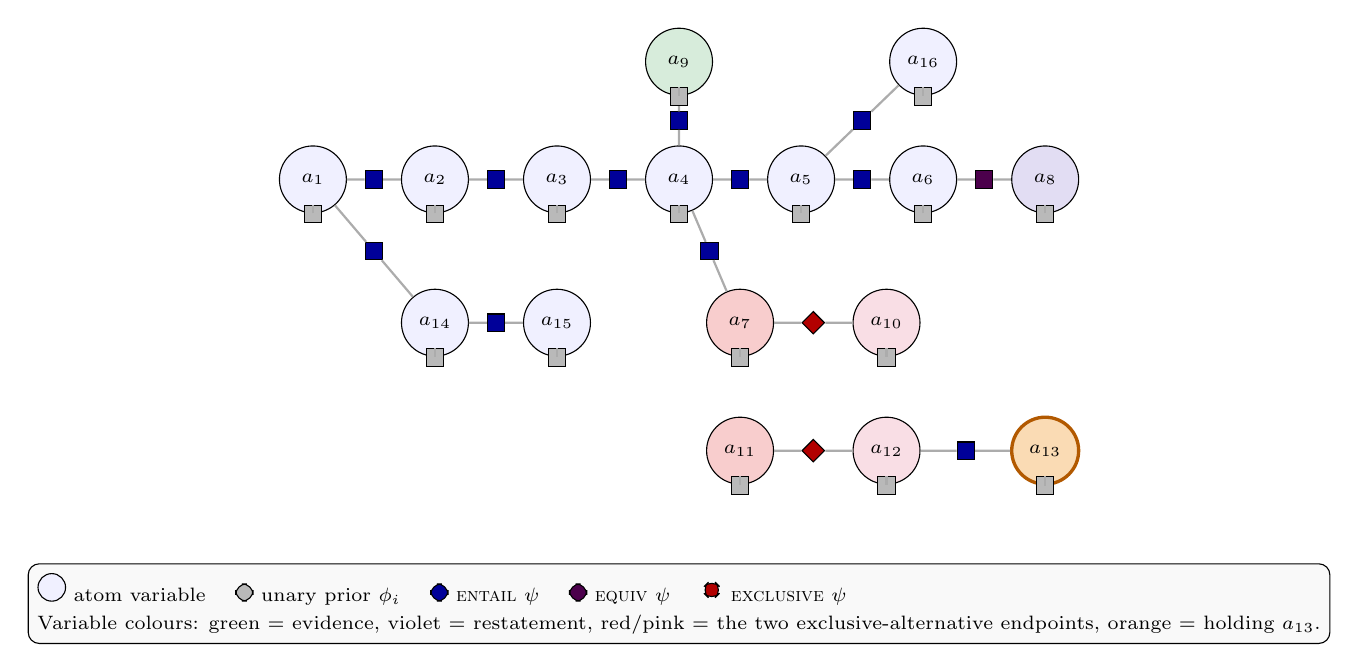
\begin{tikzpicture}[x=15.5mm,y=13mm]
  % ---- atom variables (positions mirror the relation graph) ----
  \node[var]  (a1) at (0,3)   {$a_1$};
  \node[var]  (a2) at (1,3)   {$a_2$};
  \node[var]  (a3) at (2,3)   {$a_3$};
  \node[var]  (a4) at (3,3)   {$a_4$};
  \node[var]  (a5) at (4,3)   {$a_5$};
  \node[var]  (a6) at (5,3)   {$a_6$};
  \node[varQ] (a8) at (6,3)   {$a_8$};
  \node[varE] (a9) at (3,4.15){$a_9$};
  \node[var]  (a16)at (5,4.15){$a_{16}$};
  \node[var]  (a14)at (1,1.6) {$a_{14}$};
  \node[var]  (a15)at (2,1.6) {$a_{15}$};
  \node[varCA](a7) at (3.5,1.6){$a_7$};
  \node[varCB](a10)at (4.7,1.6){$a_{10}$};
  \node[varCA](a11)at (3.5,0.35){$a_{11}$};
  \node[varCB](a12)at (4.7,0.35){$a_{12}$};
  \node[varH] (a13)at (6,0.35) {$a_{13}$};

  % ---- pairwise factors (square between the two vars) ----
  \newcommand{\pf}[4]{% #1 style #2 name #3 nodeA #4 nodeB
    \node[#1] (#2) at ($(#3)!0.5!(#4)$) {};
    \draw[link] (#3)--(#2); \draw[link] (#2)--(#4);}
  \pf{efac}{f12}{a1}{a2}
  \pf{efac}{f23}{a2}{a3}
  \pf{efac}{f34}{a3}{a4}
  \pf{efac}{f45}{a4}{a5}
  \pf{efac}{f56}{a5}{a6}
  \pf{qfac}{f68}{a6}{a8}
  \pf{efac}{f94}{a9}{a4}
  \pf{efac}{f47}{a4}{a7}
  \pf{efac}{f516}{a5}{a16}
  \pf{efac}{f114}{a1}{a14}
  \pf{efac}{f1415}{a14}{a15}
  \pf{xfac}{f710}{a7}{a10}
  \pf{xfac}{f1112}{a11}{a12}
  \pf{efac}{f1312}{a13}{a12}

  % ---- unary prior factors (small grey square hanging off each var) ----
  \foreach \v in {a1,a2,a3,a4,a5,a6,a8,a9,a16,a14,a15,a7,a10,a11,a12,a13}{
    \node[ufac] (u\v) at ($(\v)+(0,-0.34)$) {};
    \draw[link] (\v)--(u\v);
  }

  % ---- legend ----
  \node[draw,fill=gray!5,rounded corners,anchor=north,align=left,
        font=\scriptsize] at (3,-0.75) {
    \tikz\node[var,minimum size=3.5mm]{};~atom variable \quad
    \tikz\node[ufac]{};~unary prior $\phi_i$ \quad
    \tikz\node[efac]{};~\textsc{entail} $\psi$ \quad
    \tikz\node[qfac]{};~\textsc{equiv} $\psi$ \quad
    \tikz\node[xfac]{};~\textsc{exclusive} $\psi$\\[2pt]
    Variable colours: green $=$ evidence, violet $=$ restatement, red/pink $=$ the two
    exclusive-alternative endpoints, orange $=$ holding $a_{13}$.};
\end{tikzpicture}
\caption{The AeroParts response as a factor graph (the Markov network of
Eq.~\eqref{eq:joint}). Every atom has a unary prior factor; every mined relation is one
pairwise factor. The two red diamonds are the \textsc{exclusive} (exactly-one) conflict
factors; the strong one, $\psi_{7,10}$, is the coherence defect.}
\label{fig:mrf}
\end{figure}

% =====================================================================================
\section{The Logical Coherence Score}
\label{sec:lcs}

\subsection{Requirements}
An LCS for the MRF should be: (R1) a genuine functional of the joint
$P(\mathbf a)$ in Eq.~\eqref{eq:joint}; (R2) valued in $[0,1]$ and interpretable;
(R3) \emph{monotone} --- resolving/removing a contradiction must not decrease it;
(R4) contradiction-sensitive without hand-tuned constants; (R5) computable from what Merlin
already returns.

\subsection{Candidates considered}
Let $q_i=P(a_i{=}1)$ be the posterior marginals from inference on
Eq.~\eqref{eq:joint}.
\begin{enumerate}[leftmargin=*,label=(\alph*)]
  \item \textbf{Mean marginal support} $\ \mathrm{LCS}=\frac1n\sum_i q_i$.
  \item \textbf{Consistency probability} $\ P\big(\bigwedge_{r:\ \tau_r\in\{\textsc{contradict},\textsc{exclusive}\}}\neg(a_{s_r}\wedge a_{t_r})\big)$ (no conflict coupling has both endpoints true).
  \item \textbf{Reified coherence node} $P(R{=}1)$ for an added variable $R$ tied to relation
        satisfaction.
  \item \textbf{Normalized log-partition} $\big(\log Z - \log Z_{\min}\big)/\big(\log Z_{\max}-\log Z_{\min}\big)$.
\end{enumerate}
We evaluated all four by exact inference across a family of variants
(Table~\ref{tab:variants}). Findings: (b) is \emph{non-monotone} under the concession
discount --- softening a contradiction makes both endpoints co-occur \emph{more}, so
``consistency'' can fall even as coherence rises; (c) required a tuning constant and, in
several natural parameterizations, saturated or inverted under the same discount; (d) is
monotone and very contradiction-sensitive but needs a reference pair $Z_{\min},Z_{\max}$ to
land in $[0,1]$. Only (a) satisfies R1--R5 with no free constants. Section~\ref{sec:others}
develops (b), (c), and (d) in full --- how each is computed, its exact behaviour on the
example, and (for the reified node) its network construction --- and explains \emph{why}
each falls short of (a).

\subsection{Definition (selected)}
\begin{equation}
  \boxed{\ \ \mathrm{LCS}(y)\;=\;\frac{1}{n}\sum_{i=1}^{n} P(a_i{=}1)\ \ }
  \label{eq:lcs}
\end{equation}
the \textbf{mean posterior marginal support} of the atoms under the coherence MRF. It is
exactly the FactReasoner ``precision-style'' aggregate, reused: Merlin already returns the
$P(a_i)$ (MAR task), so the LCS is a one-line reduction. Interpretation: the expected
fraction of the response's atoms that the argument, taken as a whole, \emph{upholds}. A
conflict drives the losing endpoint's marginal down (in the example
$q_{10}{:}0.5\!\to\!0.40$), which lowers the mean; a satisfied entailment chain lifts its
members, which raises it.

\paragraph{Reported diagnostics.} Alongside the scalar we report, for transparency:
the per-atom marginals; the count of atoms dragged below their prior; the average
normalized entropy $\mathcal E=\frac1n\sum_i H_2(q_i)$ (FactReasoner's measure, lower is more
decisive); and the normalized $\log Z$ (candidate (d)) as a contradiction-sensitivity gauge.
These are companions, not the headline number.

% =====================================================================================
\section{The other candidate scores, in detail}
\label{sec:others}

We selected (a) mean marginal support, but the three rejected candidates are instructive:
(b) and (d) are the two natural ways to read coherence off the joint \emph{directly}, and
(c) is the most principled attempt at a single ``is-it-coherent?'' probability. This section
gives each its full construction, computation, and exact behaviour on the AeroParts family,
and pins down the failure mode. Table~\ref{tab:allcands} collects the numbers; they use the
five variants of Section~\ref{sec:change} (from least to most coherent:
\emph{worse}\,$<$\,\emph{base}\,$<$\,\emph{concession}\,$<$\,\emph{fixcasualty}\,$<$\,%
\emph{coherent}).

\begin{table}[h]\centering\small
\renewcommand{\arraystretch}{1.15}
\begin{tabular}{@{}lccccc@{}}
\toprule
\textbf{Variant} & (a) mean supp. & (b) $P(\text{cons})$ & (c) $P(R{=}1)$ & (d) $\log Z$ & (d) norm.\\
\midrule
worse        & $0.586$ & $0.738$ & $0.116$ & $-10.54$ & $0.68$\\
base         & $0.607$ & $0.828$ & $0.148$ & $-9.64$  & $0.78$\\
concession   & $0.612$ & $\mathbf{0.666}$ & $\mathbf{0.134}$ & $-9.64$ & $0.80$\\
fixcasualty  & $0.613$ & $0.865$ & $0.156$ & $-8.95$  & $0.89$\\
coherent     & $0.620$ & $1.000$ & $0.181$ & $-8.25$  & $1.00$\\
\midrule
\textbf{monotone?} & \textbf{yes} & no (bold) & no (bold) & \textbf{yes} & \textbf{yes}\\
\bottomrule
\end{tabular}
\caption{All four candidate scores across the coherence-ordered family (exact, $2^{16}$
worlds). Only (a) and (d) are monotone; (b) and (c) both \emph{dip} at the \emph{concession}
variant (bold) --- the shared quirk explained in Section~\ref{sec:quirk}. Candidate (c) uses
the noisy-AND reified node with $\rho{=}0.5$.}
\label{tab:allcands}
\end{table}

% -------------------------------------------------------------------------------------
\subsection{(b) Consistency probability}
\label{sec:consistency}

\paragraph{What it is.} The probability, under the joint $P(\mathbf a)$, that \emph{no}
conflict coupling is jointly active --- i.e.\ for every \textsc{contradict} \emph{or}
\textsc{exclusive} edge $r=(s,t)$ not both endpoints are true:
\begin{equation}
  \mathrm{LCS}_{\text{(b)}}
  \;=\;
  P\!\Big(\textstyle\bigwedge_{r:\,\tau_r\in\{\textsc{contradict},\textsc{exclusive}\}}\ \neg\big(a_{s_r}\wedge a_{t_r}\big)\Big)
  \;=\;
  \frac{1}{Z}\sum_{\mathbf a}\ \mathbb 1\!\big[\text{no conflict active in }\mathbf a\big]
  \prod_i\phi_i\!\prod_r\psi_r .
  \label{eq:cons}
\end{equation}
(For \textsc{exclusive} we take ``active'' as the both-true world, the incoherent half of the
exclusion; the both-false half is a separate, milder defect the marginals already see.)

\paragraph{How it is computed.} It is the marginal of a derived event, so it needs no new
factors: either (i) sum the joint over the worlds satisfying the indicator (the brute-force
oracle), or (ii) in production, add \emph{one} deterministic AND-style query variable
$U=\bigvee_r (a_{s_r}\wedge a_{t_r})$ and read $P(U{=}0)$ from Merlin. On the example
$\mathrm{LCS}_{\text{(b)}}$ runs $0.738\to0.828\to\mathbf{0.666}\to0.865\to1.000$.

\paragraph{Why it is rejected.} It is \emph{not monotone}: the \emph{concession} variant
\emph{drops} to $0.67$ even though softening the resolved tension makes the response
\emph{more} coherent. Root cause in Section~\ref{sec:quirk}. It also ignores
entailment/equivalence entirely --- a response with a beautifully satisfied causal spine and
a response that is a disconnected bag of atoms score identically at $1.0$ if neither has an
active contradiction. Good as a \emph{diagnostic} ("is there a live contradiction?"), poor
as the headline score.

% -------------------------------------------------------------------------------------
\subsection{(c) Reified coherence node $P(R{=}1)$}
\label{sec:reified}

\paragraph{What it is.} Add one binary variable $R$ ("the response is coherent") to the
network and let every relation \emph{vote} on it, so that a single marginal $P(R{=}1)$
summarizes global coherence. This is the most direct realization of "give me one number
that means coherent."

\paragraph{Construction (noisy-AND over relation satisfaction).} We attach $R$ to each
relation $r$ by a three-way factor $h_r(R,a_{s_r},a_{t_r})$ that, in the $R{=}1$ branch,
charges the relation's confidence $p_r$ whenever it is \emph{violated}, and in the $R{=}0$
branch is flat:
\begin{equation}
  h_r(R{=}1,\,x,\,y)=
  \begin{cases}
    1, & \text{$r$ satisfied at }(x,y)\\[2pt]
    1-p_r, & \text{$r$ violated at }(x,y)
  \end{cases}
  \qquad
  h_r(R{=}0,\,x,\,y)=1,
  \label{eq:reified}
\end{equation}
with ``violated'' meaning $x{=}1,y{=}0$ (\textsc{entail}), $x\neq y$ (\textsc{equiv}),
$x{=}y{=}1$ (\textsc{contradict}), $x{=}y$ (\textsc{exclusive}, either same-value world), or
$x{=}y{=}0$ (\textsc{co-nec}) --- the same conditions as the diagnostics. A Bernoulli
prior $\rho$ on $R$ completes it. The reified network's joint is
\begin{equation}
  P(\mathbf a,R)\;=\;\frac1{Z'}\,\rho^{R}(1-\rho)^{1-R}
  \Big(\prod_i\phi_i\!\prod_r\psi_r\Big)\prod_r h_r(R,a_{s_r},a_{t_r}),
  \label{eq:reified-joint}
\end{equation}
and the score is the marginal
\(
  \mathrm{LCS}_{\text{(c)}}=P(R{=}1)=\sum_{\mathbf a}P(\mathbf a,R{=}1).
\)
Intuitively, $R{=}1$ is a hypothesis that must ``pay'' a factor $1-p_r$ for every confident
relation the world breaks; the more (and the more confident) the broken relations, the less
posterior mass $R{=}1$ retains. Because each relation contributes an independent factor to
$R$ given the atoms, this is a \emph{noisy-AND}: $R{=}1$ is favoured only when
(approximately) \emph{all} relations are honoured.

Figure~\ref{fig:reified-graph} shows the augmented factor graph: it is the network of
Figure~\ref{fig:mrf} plus the node $R$, its prior factor, and one $h_r$ factor per relation
(so $R$ has degree $|R|$). Figure~\ref{fig:reified-calc} traces the computation on a minimal
3-atom subnet so the mechanism is fully visible.

\begin{figure}[h]\centering
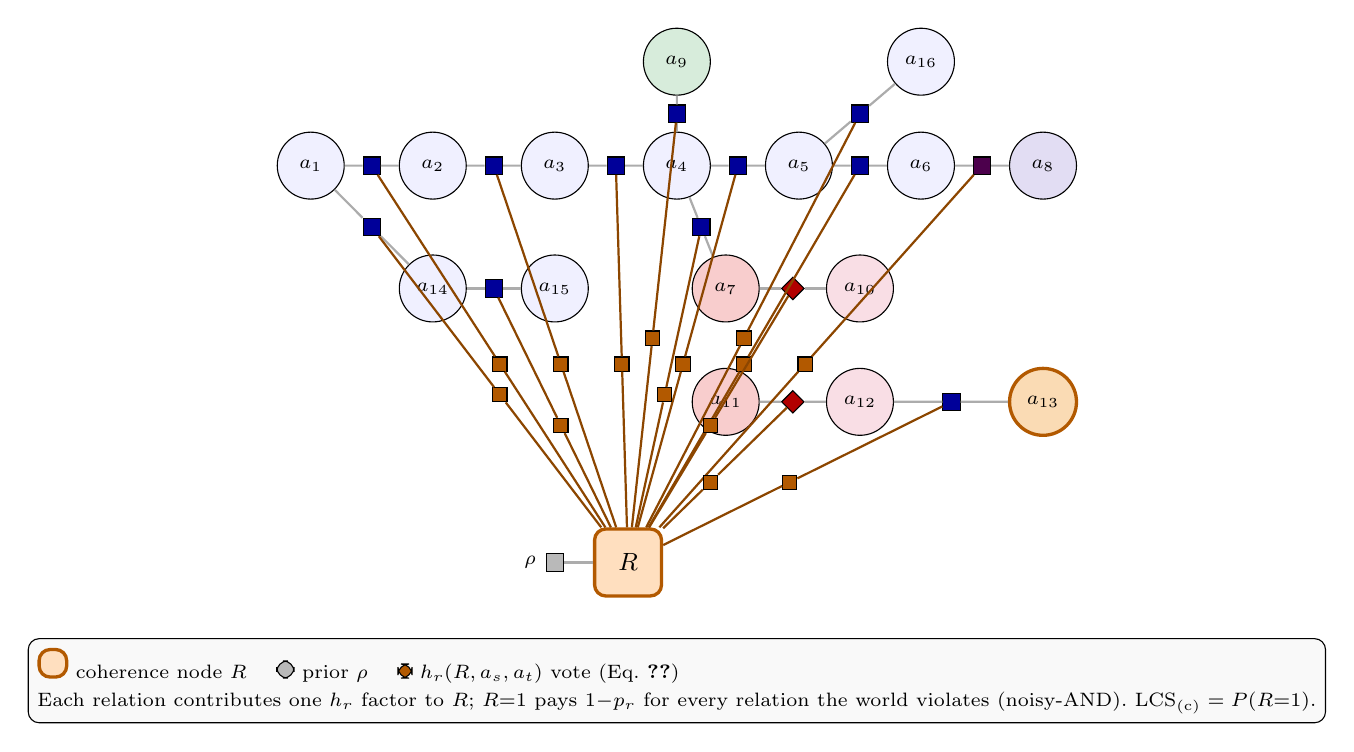
\begin{tikzpicture}[x=15.5mm,y=12mm]
  % abbreviated atom layout (same positions as Fig 1, fewer labels for clarity)
  \node[var]  (a1) at (0,3)   {$a_1$};
  \node[var]  (a2) at (1,3)   {$a_2$};
  \node[var]  (a3) at (2,3)   {$a_3$};
  \node[var]  (a4) at (3,3)   {$a_4$};
  \node[var]  (a5) at (4,3)   {$a_5$};
  \node[var]  (a6) at (5,3)   {$a_6$};
  \node[varQ] (a8) at (6,3)   {$a_8$};
  \node[varE] (a9) at (3,4.1) {$a_9$};
  \node[var]  (a16)at (5,4.1) {$a_{16}$};
  \node[var]  (a14)at (1,1.7) {$a_{14}$};
  \node[var]  (a15)at (2,1.7) {$a_{15}$};
  \node[varCA](a7) at (3.4,1.7){$a_7$};
  \node[varCB](a10)at (4.5,1.7){$a_{10}$};
  \node[varCA](a11)at (3.4,0.5){$a_{11}$};
  \node[varCB](a12)at (4.5,0.5){$a_{12}$};
  \node[varH] (a13)at (6,0.5)  {$a_{13}$};

  % relation factors (small, just markers -- endpoints omitted to keep the R fan readable)
  \newcommand{\rf}[4]{\node[#1] (#2) at ($(#3)!0.5!(#4)$) {};
     \draw[link] (#3)--(#2); \draw[link] (#2)--(#4);}
  \rf{efac}{f12}{a1}{a2}\rf{efac}{f23}{a2}{a3}\rf{efac}{f34}{a3}{a4}
  \rf{efac}{f45}{a4}{a5}\rf{efac}{f56}{a5}{a6}\rf{qfac}{f68}{a6}{a8}
  \rf{efac}{f94}{a9}{a4}\rf{efac}{f47}{a4}{a7}\rf{efac}{f516}{a5}{a16}
  \rf{efac}{f114}{a1}{a14}\rf{efac}{f1415}{a14}{a15}
  \rf{xfac}{f710}{a7}{a10}\rf{xfac}{f1112}{a11}{a12}\rf{efac}{f1312}{a13}{a12}

  % the reified node R, bottom-centre, with its prior factor
  \node[coh] (R) at (2.6,-1.2) {$R$};
  \node[ufac] (rho) at ($(R)+(-0.6,0)$) {}; \draw[link] (R)--(rho);
  \node[font=\scriptsize,left] at (rho.west) {$\rho$};

  % h_r factors: draw R connected to the relation factors it votes with.
  % To keep it legible, route R to each relation-factor square (grey diamond = h_r).
  \foreach \ff in {f12,f23,f34,f45,f56,f68,f94,f47,f516,f114,f1415,f710,f1112,f1312}{
    \node[fac,fill=orange!70!black,minimum size=1.8mm] (h\ff) at ($(\ff)!0.5!(R)$) {};
    \draw[link,orange!55!black] (\ff)-- (h\ff);
    \draw[link,orange!55!black] (h\ff) -- (R);
  }

  \node[draw,fill=gray!5,rounded corners,anchor=north,align=left,
        font=\scriptsize] at (3,-2.0) {
    \tikz\node[coh,minimum size=3.5mm]{};~coherence node $R$ \quad
    \tikz\node[ufac]{};~prior $\rho$ \quad
    \tikz\node[fac,fill=orange!70!black,minimum size=1.8mm]{};~$h_r(R,a_s,a_t)$ vote (Eq.~\ref{eq:reified}) \\[2pt]
    Each relation contributes one $h_r$ factor to $R$; $R{=}1$ pays $1{-}p_r$ for every
    relation the world violates (noisy-AND). $\mathrm{LCS}_{\text{(c)}}=P(R{=}1)$.};
\end{tikzpicture}
\caption{The reified network: Figure~\ref{fig:mrf} augmented with the coherence node $R$
(orange), its prior $\rho$, and one orange $h_r$ vote-factor per relation. $R$ has degree
$|R|$; every relation gets a say in whether the response is coherent.}
\label{fig:reified-graph}
\end{figure}

\begin{figure}[h]\centering
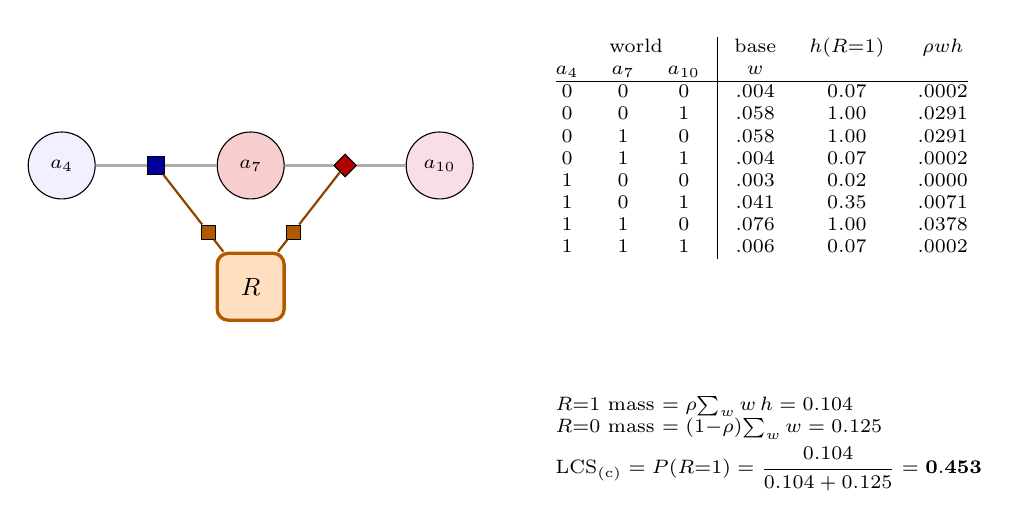
\begin{tikzpicture}[x=15mm,y=11mm]
  % minimal subnet: a4 ->(entail .65) a7 (excl .93) a10
  \node[var]  (a4) at (0,0) {$a_4$};
  \node[varCA](a7) at (1.6,0){$a_7$};
  \node[varCB](a10)at (3.2,0){$a_{10}$};
  \node[efac] (e) at (0.8,0){}; \draw[link](a4)--(e);\draw[link](e)--(a7);
  \node[xfac] (c) at (2.4,0){}; \draw[link](a7)--(c);\draw[link](c)--(a10);
  \node[coh]  (R) at (1.6,-1.4){$R$};
  \node[fac,fill=orange!70!black,minimum size=1.8mm] (he) at ($(e)!0.55!(R)$){};
  \node[fac,fill=orange!70!black,minimum size=1.8mm] (hc) at ($(c)!0.55!(R)$){};
  \draw[link,orange!55!black](e)--(he);\draw[link,orange!55!black](he)--(R);
  \draw[link,orange!55!black](c)--(hc);\draw[link,orange!55!black](hc)--(R);
  % table
  \node[anchor=west,align=left,font=\scriptsize] at (4.1,0.2){
    \begin{tabular}{@{}ccc|ccc@{}}
    \multicolumn{3}{c|}{world} & base & $h(R{=}1)$ & $\rho w h$\\
    $a_4$&$a_7$&$a_{10}$ & $w$ & & \\ \hline
    0&0&0 & .004 & $0.07$ & .0002\\
    0&0&1 & .058 & $1.00$ & .0291\\
    0&1&0 & .058 & $1.00$ & .0291\\
    0&1&1 & .004 & $0.07$ & .0002\\
    1&0&0 & .003 & $0.02$ & .0000\\
    1&0&1 & .041 & $0.35$ & .0071\\
    1&1&0 & .076 & $1.00$ & .0378\\
    1&1&1 & .006 & $0.07$ & .0002\\
    \end{tabular}};
  \node[anchor=north west,align=left,font=\scriptsize] at (4.1,-2.55)
    {$R{=}1$ mass $=\rho\!\sum_w w\,h = 0.104$\\
     $R{=}0$ mass $=(1{-}\rho)\!\sum_w w = 0.125$\\[2pt]
     $\mathrm{LCS}_{\text{(c)}}=P(R{=}1)=\dfrac{0.104}{0.104+0.125}=\mathbf{0.453}$};
\end{tikzpicture}
\caption{Reified computation on a 3-atom subnet ($a_4\!\to\!a_7$, \textsc{entail} $.65$;
$a_7\!\oplus\!a_{10}$, \textsc{exclusive} $.93$), $\rho{=}0.5$. Worlds that break the strong
exclusion --- \emph{both} same-value rows $a_7{=}a_{10}$ (both-true \emph{and} both-false) ---
get $h{=}1{-}.93{=}.07$; the world that also breaks the entailment ($a_4{=}1,a_7{=}0,a_{10}{=}0$)
compounds to $h{=}.35\!\times\!.07{=}.02$; $R{=}1$'s posterior mass is suppressed accordingly.
Summing gives $P(R{=}1)=0.453$.}
\label{fig:reified-calc}
\end{figure}

\paragraph{Behaviour and why it is rejected.} $P(R{=}1)$ \emph{is} discriminative and
monotone for add/remove edits ($0.116$ \emph{worse} $\to 0.181$ \emph{coherent}) and it
folds in \emph{all} relation types (unlike (b)). But it inherits the same
\emph{concession non-monotonicity} ($0.148$ \emph{base} $\to 0.134$ \emph{concession}) --- it
reads ``is the relation active'' through the same lens as (b) --- and it introduces a free
hyper-parameter $\rho$ (and, in richer variants, per-relation vote weights) that must be
calibrated. A single tuned constant standing between the model and the headline number is
exactly what we wanted to avoid; (a) needs none. We therefore keep the reified node as an
\emph{optional} interpretable read-out, not the definition.

% -------------------------------------------------------------------------------------
\subsection{(d) Normalized log-partition}
\label{sec:logz}

\paragraph{What it is.} The (log) partition function $Z=\sum_{\mathbf a}\prod_i\phi_i\prod_r\psi_r$
measures how much total probability mass the factors let the network retain. Entailment and
equivalence factors that are jointly satisfiable \emph{raise} $Z$; an active conflict factor
(\textsc{contradict} or \textsc{exclusive}) caps mass on the offending configurations and
\emph{lowers} it. Rescaled to $[0,1]$ against two references,
\begin{equation}
  \mathrm{LCS}_{\text{(d)}}
  \;=\;
  \frac{\log Z - \log Z_{\min}}{\log Z_{\max}-\log Z_{\min}} ,
  \label{eq:logz}
\end{equation}
with $Z_{\max}$ the same network with all conflict factors (\textsc{contradict} and
\textsc{exclusive}) removed (the maximally-coherent reference; removing constraint factors
only adds mass, so $\log Z\le\log Z_{\max}$).

\paragraph{The floor $Z_{\min}$: the MAP-world mass.} A graded $[0,1]$ score needs a valid
\emph{lower} reference. We use the mass of the single most-probable world,
\begin{equation}
  Z_{\min}\;=\;\max_{\mathbf a}\ \prod_i\phi_i(a_i)\prod_r\psi_r(\mathbf a),
  \qquad
  \log Z_{\min}\;=\;\max_{\mathbf a}\ \log\mathrm{mass}(\mathbf a),
  \label{eq:zmin}
\end{equation}
i.e.\ the mass of the \textsc{map} configuration. This is a \emph{provable} lower bound:
$Z$ is a sum of non-negative terms, so it is at least its single largest term,
$Z=\sum_{\mathbf a}\mathrm{mass}(\mathbf a)\ge\max_{\mathbf a}\mathrm{mass}(\mathbf a)=Z_{\min}$,
hence $\log Z_{\min}\le\log Z\le\log Z_{\max}$ for \emph{every} network, by construction rather
than by luck. It is also coherence-graded: the \textsc{map} world is the network's best-case
reading (the assignment satisfying as many relations as possible), so when contradictions are
weak some world satisfies almost everything and $\log Z_{\min}$ sits near $\log Z$, whereas
when contradictions are strong and mutually binding \emph{even the best world} must violate
some of them, dragging $\log Z_{\min}$ down with coherence. The score then reads: $1.0$ when
the base already sits at the contradiction-free ceiling ($\log Z=\log Z_{\max}$), tending to
$0$ as the base collapses onto its own single-world floor.

\emph{Why not simpler floors.} Two skeleton-derived candidates fail for the row-stochastic
with-priors tables of \S\ref{sec:tables}: ``retype every edge to a \textsc{contradict}'' and
``saturate the existing \textsc{contradict} factors to $p{=}1$'' are both \emph{not} valid
lower bounds. The with-priors contradiction factor is row-stochastic (each source-state row
sums to $1$), so an isolated contradiction removes no mass and only bites where it competes
with other factors over shared atoms; a mass-\emph{concentrating} entailment backbone plus
several soft contradictions can therefore drive the base $\log Z$ \emph{below} either
construction (empirically the base fell below both on a third of real graphs). The
\textsc{map}-world mass sidesteps this entirely --- it is a term of the actual sum, so it
cannot exceed it.

\paragraph{How it is computed.} $Z$ is exactly the normalizing constant of the joint;
Merlin's \textbf{PR} (partition) task returns $\log Z$, and its \textbf{MAP} task returns
$\log Z_{\min}$ (the log-mass of the argmax configuration) --- one extra query on the
\emph{same} base network, plus one PR run on the contradiction-free network for
$\log Z_{\max}$. On the \emph{AeroParts} base network (exact, over $2^{16}$ worlds)
$\log Z=-9.64$, $\log Z_{\min}=-14.69$, $\log Z_{\max}=-8.25$, giving
$\mathrm{LCS}_{\text{(d)}}=(-9.64+14.69)/(-8.25+14.69)=\mathbf{0.78}$; the conflict-free
variant has $\log Z=\log Z_{\max}$ and normalizes to $\mathbf{1.00}$. Across the
coherence-ordered family of Section~\ref{sec:change} the normalized score runs
$0.68\to0.78\to0.80\to0.89\to1.00$ (Table~\ref{tab:allcands}) --- \emph{cleanly monotone} and
genuinely graded in $[0,1]$; raw $\log Z$ is likewise monotone and the most
conflict-sensitive of the four candidates (a single confident conflict costs
$\approx$ a full nat).

\paragraph{Status: a graded diagnostic, still not the headline.} With the \textsc{map} floor,
$\mathrm{LCS}_{\text{(d)}}$ is a genuine $[0,1]$ score (it was previously degenerate under the
$Z_{\min}=$ base-network choice, which forced every contradiction-bearing graph to $0$). It
remains a \emph{diagnostic} rather than the headline for two reasons unchanged by the fix: it
needs the reference pair $(Z_{\min},Z_{\max})$ --- two extra inference runs (a MAP query and a
PR run on a modified network) --- and it is a whole-network quantity with no per-atom
decomposition, so it cannot say \emph{which} atoms the incoherence attaches to. We therefore
keep the mean marginal support (a) as the headline and report the normalized $\log Z$ (with
its $Z_{\min},Z_{\max}$ endpoints) alongside raw $\log Z$ as the contradiction-sensitivity
companion, as in Table~\ref{tab:variants}.

% -------------------------------------------------------------------------------------
\subsection{The shared concession quirk}
\label{sec:quirk}

Candidates (b) and (c) both dip at the \emph{concession} variant; (a) and (d) do not. The
reason is precise. The concession edit \emph{softens} the resolved conflict
$a_{11}\!\oplus\!a_{12}$ from $p{=}0.80$ to $p{=}0.55$. A weaker \textsc{exclusive} factor
puts \emph{more} mass on the both-true cell (its $(1,1)$ entry is $1{-}p$, exactly as for
\textsc{contradict}): for a lone edge with uniform priors the with-priors table gives
\[
  P(a_{11}{=}1,a_{12}{=}1)\ =\ 0.10\ \ (p{=}0.80)\qquad\longrightarrow\qquad 0.225\ \ (p{=}0.55).
\]
Scores that read ``\emph{is} the conflict active'' --- (b) counts the event, (c) charges
$1{-}p$ for it --- therefore register the softened edge as \emph{more often active}, and dip.
Scores that read ``\emph{how strongly do we believe} each atom'' --- (a) the marginals, (d)
the mass --- correctly see the softening as \emph{less} suppression and rise. This is the
crux of the selection: a coherence score should track \emph{belief}, not \emph{event
activity}, and (a) does so with no tunable constant. The concession discount itself remains
the right modeling move (Eq.~\ref{eq:concession}); the lesson is only about which read-out
sits on top of it.

% =====================================================================================
\section{Baseline algorithm to compute the LCS}
\label{sec:algo}

Algorithm~\ref{alg:lcs} is the baseline. It reuses the shipped
\texttt{FactGraph}\,$\to$\,\texttt{MarkovNetwork}\,$\to$\,Merlin path; the only new code is
Level-2 compilation (Section~\ref{sec:level2}) and the final reduction
(Eq.~\eqref{eq:lcs}).

\begin{figure}[h]
\centering
\fbox{\parbox{0.94\textwidth}{\small
\textbf{Algorithm 1: \textsc{ComputeLCS}$(y)$}\\[2pt]
\textbf{Input:} response $y$; miner $\mathcal M$; discount $\lambda$; prior $\pi$.\\
\textbf{Output:} $\mathrm{LCS}\in[0,1]$, marginals $\{q_i\}$, diagnostics.
\begin{enumerate}[leftmargin=1.4em,nosep,label=\arabic*.]
  \item $A \leftarrow \textsc{AtomizeAndDecontextualize}(y)$
        \hfill// reuse Atomizer + Reviser
  \item $C \leftarrow \textsc{CandidatePairs}(A)$
        \hfill// order-window $+$ similarity/entity prune (avoid full $O(n^2)$)
  \item $R \leftarrow \varnothing$
  \item \textbf{for each} $(a_i,a_j)\in C$:
    \begin{enumerate}[leftmargin=1.4em,nosep,label=\alph*.]
      \item $(\text{sense},\ \tau,\ p)\leftarrow \mathcal M(a_i,a_j)$
            \hfill// Level-2 sense $+$ Level-1 $\tau$ $+$ confidence (logprobs / SIMBA-UQ)
      \item \textbf{if} $\tau=\textsc{none}$ \textbf{then continue}
      \item \textbf{if} sense $=$ Concession \textbf{and} $\exists\,h$ resolving $(i,j)$:
            $\ p \leftarrow p\,(1-\lambda\,\pi_h)$ \hfill// Eq.~\eqref{eq:concession}
      \item $R \leftarrow R\cup\{(i,j,\tau,p)\}$
    \end{enumerate}
  \item $G \leftarrow \textsc{FactGraph}(A,\,R)$ with every edge \texttt{link="atom\_atom"}
  \item $\mathcal N \leftarrow \textsc{BuildMarkovNetwork}(G)$:
        \hfill// \texttt{use\_priors}\,$=$\,\textbf{True}
        \begin{enumerate}[leftmargin=1.4em,nosep,label=\alph*.]
          \item add node $a_i$ with unary factor $[\,1-\pi,\ \pi\,]$ for all $i$
          \item add pairwise factor $\psi_r$ per Table~\ref{tab:tables} (with-priors) for all $r\in R$
        \end{enumerate}
  \item $\{q_i\} \leftarrow \textsc{Merlin}(\mathcal N,\ \text{task}{=}\text{MAR})$
        \hfill// posterior marginals $P(a_i{=}1)$
  \item $\mathrm{LCS} \leftarrow \frac1n\sum_i q_i$
        \hfill// Eq.~\eqref{eq:lcs}
  \item \textbf{return} $\mathrm{LCS}$, $\{q_i\}$, diagnostics$\big(\#\{q_i{<}\pi\},\ \mathcal E,\ \log Z\big)$
\end{enumerate}
}}
\label{alg:lcs}
\end{figure}

\paragraph{Complexity.} Steps 1--4 dominate wall-clock: $|C|$ miner calls, kept near-linear
by the pruning in step~2 (windowing $+$ embedding/entity gate) rather than the naive
$\binom n2$. Step~8 is Merlin WMB (i-bound~6), sub-second for the graph sizes seen in
practice; exact inference is feasible only for small $n$ (the $2^{16}$ brute force used for
this document's numbers is a \emph{validation} oracle, not the production path).

% =====================================================================================
\section{How the LCS changes: base vs.\ coherent rewrite}
\label{sec:change}

We now exercise requirement R3. Table~\ref{tab:variants} reports the exact LCS across a
family of edits to the same response, ordered from least to most coherent.

\begin{table}[h]\centering\small
\renewcommand{\arraystretch}{1.1}
\begin{tabular}{@{}p{6.4cm}ccc@{}}
\toprule
\textbf{Variant} & \textbf{LCS} (Eq.~\ref{eq:lcs}) & \textbf{$\#\{q_i{<}\pi\}$} & \textbf{$\log Z$}\\
\midrule
\emph{worse}: add a spurious contradiction $a_3\!\neq\!a_{12}$ ($p{=}.85$) & $0.586$ & 4 & $-10.54$\\
\textbf{base}: both conflicts present                                       & $0.607$ & 3 & $-9.64$\\
concession resolved: $a_{11}\!\oplus\!a_{12}$ discounted $.80\!\to\!.55$      & $0.612$ & 2 & $-9.64$\\
fix casualty conflict only: drop $a_7\!\oplus\!a_{10}$                        & $0.613$ & 1 & $-8.95$\\
\textbf{coherent rewrite}: remove both conflicts                             & $0.620$ & 0 & $-8.25$\\
\bottomrule
\end{tabular}
\caption{Exact LCS across coherence-changing edits (with-priors MRF, $\pi{=}0.5$, $2^{16}$
worlds). LCS is \emph{monotone}: it falls when a conflict is added and rises as tensions
are resolved or removed. The diagnostics move in lockstep --- the below-prior count drops
$4\!\to\!0$ and $\log Z$ rises $-10.54\!\to\!-8.25$.}
\label{tab:variants}
\end{table}

\paragraph{Where the change comes from.} Table~\ref{tab:margchange} shows the per-atom
marginals for the base vs.\ the coherent rewrite. Only the atoms attached to the removed
conflicts move: the casualty pair's loser $a_{10}$ recovers $0.40\!\to\!0.50$ and the blame
loser $a_{11}$ recovers $0.40\!\to\!0.50$. (The \textsc{exclusive} coupling already keeps the
losers well off the floor at $\approx 0.40$ --- because ``neither'' is forbidden too, so
rejecting one endpoint half-supports the other --- which is why the recovery is a gentle
$0.10$ rather than the $0.26$ a bare \textsc{contradict} would show; $a_{12}$ is held up by
the $a_{13}\!\to\!a_{12}$ evidence link and does not move.) The entire causal backbone
($a_1$--$a_6$, $a_{14}$--$a_{16}$) is \emph{unchanged} --- coherence editing is local, exactly
as it should be. The $+0.013$ LCS gain is the averaged lift of the two freed atoms.

\begin{table}[h]\centering\small
\begin{tabular}{@{}l*{8}{c}@{}}
\toprule
      & $a_7$ & $a_{10}$ & $a_{11}$ & $a_{12}$ & $a_{13}$ & (backbone) & mean & LCS\\
\midrule
base             & .611 & \textbf{.404} & \textbf{.395} & .675 & .500 & unchanged & .607 & \textbf{0.607}\\
coherent rewrite & .611 & \textbf{.500} & \textbf{.500} & .675 & .500 & unchanged & .620 & \textbf{0.620}\\
\bottomrule
\end{tabular}
\caption{Per-atom marginals, base vs.\ coherent rewrite. Only the two conflict-loser atoms
change (bold); the backbone and the evidence-supported $a_{12}$/$a_{13}$ are untouched. The
LCS rises $0.607\!\to\!0.620$.}
\label{tab:margchange}
\end{table}

% =====================================================================================
\section{Summary}
\label{sec:summary}

\begin{itemize}[leftmargin=*]
  \item \textbf{Construction:} one binary variable per atom, one unary prior factor per
        variable, one pairwise factor per mined relation --- the shipped
        \texttt{MarkovNetwork} path, with \texttt{link="atom\_atom"} edges and the
        \textbf{with-priors} factor tables (Section~\ref{sec:tables}).
  \item \textbf{Two levels:} Level~1 couplings (\textsc{entail}/\textsc{contradict}/%
        \textsc{equiv}) map straight to factors; Level~2 discourse senses \emph{compile}
        to Level~1 plus a strength prior, with Concession the one case needing structure
        (a resolving-holding discount, Eq.~\eqref{eq:concession}).
  \item \textbf{LCS:} the mean posterior marginal support, Eq.~\eqref{eq:lcs} --- the
        MRF-native choice: monotone, in $[0,1]$, constant-free, and already returned by
        Merlin.
  \item \textbf{Algorithm:} \textsc{ComputeLCS} (Alg.~1) is a thin extension of the existing
        pipeline: add Level-2 compilation and a final averaging step.
  \item \textbf{Behaviour:} on AeroParts the LCS moves $0.586$ (worse) $\to 0.607$ (base)
        $\to 0.620$ (coherent), driven entirely by the local un-suppression of the
        conflict-attached atoms.
\end{itemize}

% =====================================================================================
\begin{thebibliography}{9}\small
\bibitem[FactReasoner]{factreasoner} R.~Marinescu et al.
  \emph{FactReasoner: A Probabilistic Approach to Long-Form Factuality Assessment for LLMs.}
  arXiv:2502.18573, 2025.
\bibitem[SIMBA-UQ]{simbauq} D.~Bhattacharjya et al.
  \emph{SIMBA-UQ: Similarity-Based Aggregation for UQ in LLMs.} Findings of EMNLP 2025,
  arXiv:2510.13836.
\bibitem[PDTB3]{pdtb3} B.~Webber, R.~Prasad, A.~Lee, A.~Joshi.
  \emph{The Penn Discourse Treebank 3.0 Annotation Manual.} LDC2019T05, 2019.
\bibitem[RST]{rst} W.~Mann, S.~Thompson. \emph{Rhetorical Structure Theory.} Text 8(3), 1988.
\bibitem[DiscoPrompt]{discoprompt} C.~Chan et al.
  \emph{DiscoPrompt: Path Prediction Prompt Tuning for Implicit Discourse Relation
  Recognition.} ACL Findings 2023, arXiv:2305.03973.
\end{thebibliography}

\end{document}
